\chapter{Introduction}
\section{Background and Motivation}

Traditionally the thermal diffusivity, otherwise referred to as the $\alpha$-value, of timber is based simply off the EN 1995:1-1-2004 or similar standards.
This research project will aim to obtain the thermal diffusivity of cross laminated SA-Pine timber by further analysing data obtained by S van der Westhuisen for his study of the samples' charring rate.

The thermal diffusivity of timber is a unobservable quantity that cannot be measured by itself, instead it is related to measurements of temperature and time through differential models. 
When heat diffusion is calculated using Finite Element methods the process is usually simplified to a linear problem \citep{Fish:2007}. 
Due to the changes in thermal diffusivity of timber with temperature, as can be seen in EN 1995:1-1-2004(pg number TODO), the diffusivity cannot be linearly modelled. 
Therefore the problem lends itself to being analysed by inversion techniques. 
The aforementioned approach will allow us to obtain information about the diffusivity based on the combination of the information assumed prior to measuring, further referred to as the prior, and the measured data. 
Using statistical inversion leads to a probability distribution that provides us with a collection of diffusivity estimates and their corresponding probabilities.


%This will be done by adjusting a finite element model created by Dr. N de Koker into a function. This function will be used in a Bayes model to solve for the temperature dependant thermal diffusivity.
\section{Aim and objectives}
During the course of the project the student will aim to meet the following objectives:
\begin{enumerate}
 \item Modify a Finite Element Model into an accurate and effective function.
 \item Compare the model data to the actual acquired data.
 \item Solve for the thermal diffusivity using Bayes' theorem of inverse problems
 \item Evaluate and explore the posterior probability distribution using the following methods:
 	\begin{enumerate}
 		\item Maximum a Posteriori
 		\item Markov-Chain Monte Carlo 	
 	\end{enumerate}
\end{enumerate}

\section{Literature Review}
This section aims to summarise the current body of knowledge available on the topic. 
The relevance to this information and the report will also be indicated. 
%after this section the reader will understand every term, idea and concept that existed prior to the undertaking of the project.
	\subsection{K- value}
	The current K-values used for the design of timber elements are taken from the EURO code (ref TODO)  
%	\begin{figure}
%	\label{kvalue_fig}
%	\begin{center}
%	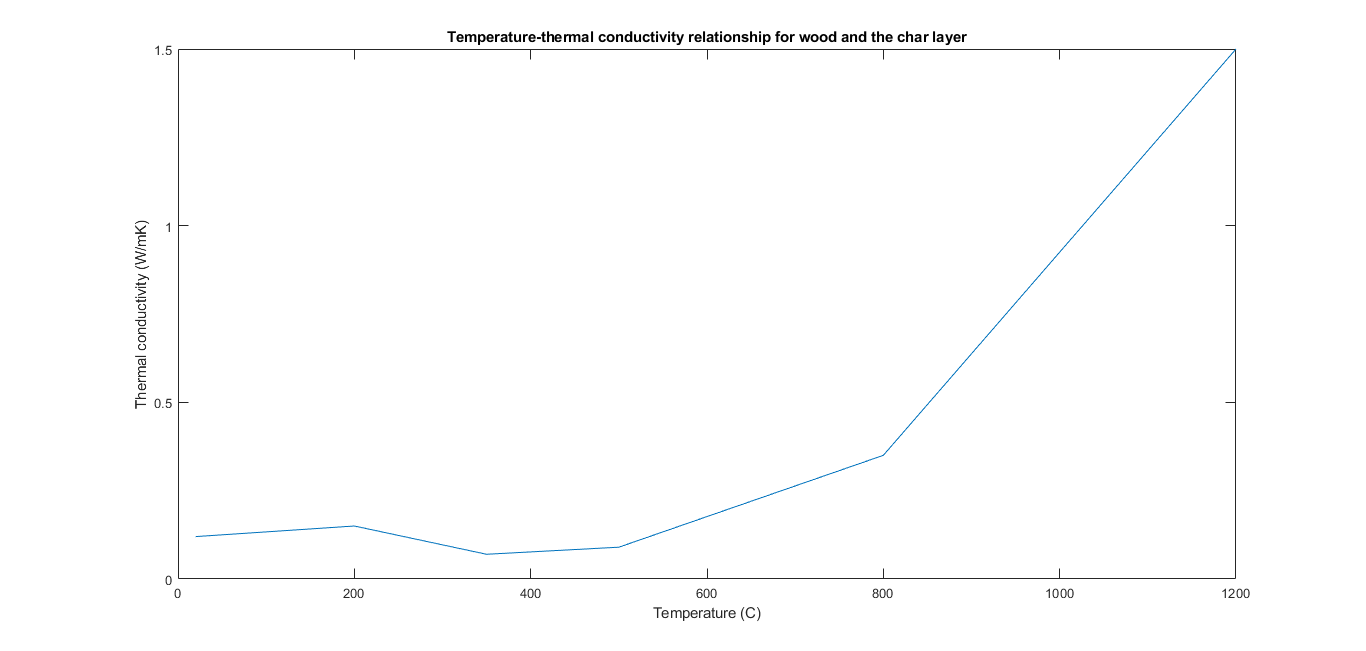
\includegraphics[width = 3]{kvalues_euro.png}
%	\end{center}
%	\end{figure}
	
	\subsection{Bayes' theorem of inverse problems}
%	Statistical and Computational Inverse problems by Kaipio and Somersalo Chapter 3
% 	The Bayesian approach to Inverse Problems Dashti and Stuart
	The method of statistical inversion is dependant on a fundamental understanding of the Bayes' theorem of inverse problems. 
	The student obtained this understanding through studying Chapter 3 of Statistical and Computational Inverse problems by \citet{Kaipo:2005}, further referred to merely as Kaipio. 
	There are four principles of Statistical inversion that is essential to the thorough understanding of these models. 
	Firstly it is the principle that any variable in the model needs to be modelled as a random variable. 
	This randomness is based on the extent of information that is available. 
	To ensure that the extent of knowledge is accurately portrayed in the model the extent of knowledge will be coded into the probability distributions assigned to the different variables. 
	Finally it needs to be understood that the solution of a statistical inversion is a posterior probability distribution.
	A generalized equation of Bayes' theorem can be seen in \ref{bayes_eq} taken from Kiapio. 
	
	\begin{equation}
	\label{bayes_eq}
	\pi_{\text{post}}(x) = \pi(x|y_{\text{observed}}) = \frac{\pi_{\text{pr}}(x) \pi(y_{\text{observed}}|x)}{\pi (y_{\text{observed}})}	
	\end{equation}
	\subsection{Heat diffusion equation}
	
	
	\begin{equation}
	\label{heat_eq}
		q = -k \frac{dT}{dx}
	\end{equation}
\section{Proposed methodology}
	\subsection{Finite Element Model}
	A one-dimensional finite element model that simulates what we expect to obtain from the fire tests based on the simplified K-values provided in EN 1995:1-1-2004 will be modified into a function.
	 This function should provide the temperature of the modelled element based on a specified location and thermal conductivity.
	\subsection{Optimization}
	\subsection{Markov Chain Monte Carlo}
	Markov Chain Monte Carlo(MCMC) is a method of integration. This will be used to determine the mean of the k-values at specific temperatures. 
	Markov Chain Monte Carlo is a method that was created by combining the concept of Monte Carlo sampling  and a Markov Chain. 
	To fully understand MCMC the methods that it was created from need to be further investigated.
		\subsubsection{Markov Chains}
		
		
		
		\subsubsection{Monte Carlo Integration}
		Monte Carlo integration is used to evaluate a probability distributuion. 
		The evaluation is done by drawing a collection of random numbers from the distribution.
		These numbers are then used a the sample and a sample mean is taken.
		The arithmetic sample mean can be used to approximate the population mean in accordance with the law of large numbers \citep{Gilks:1996} 

	
\section{Program}